%%% Ne pas modifier jusqu'à la ligne 25
\documentclass[a4paper,12pt]{book}
\usepackage[utf8]{inputenc}
\usepackage[french]{babel}
%%\usepackage{CJK}
\usepackage{yhmath}
\usepackage[left=2cm,right=2cm,top=3cm,bottom=2cm, headheight=1.5cm,headsep=1.5cm]{geometry}
%%\usepackage{CJKutf8}
\usepackage{amsfonts}
\usepackage{amsmath,amsfonts,amssymb,dsfont}
\usepackage{graphicx}
\usepackage{subfigure}
\usepackage{enumitem}		%\enumerate-resume
\usepackage[colorlinks=true,unicode={true},hyperindex=false, linkcolor=blue, urlcolor=blue]{hyperref}
\newcommand{\myref}[1]{\ref{#1} page \pageref{#1}}

\addto\captionsfrench{\def\tablename{Tableau}}  %légendes des tableaux
\renewcommand\thesection{\Roman{section}~-~} 
\renewcommand\thesubsection{\Roman{section}.\Alph{subsection}~-~} 
\renewcommand\thesubsubsection{\Roman{section}.\Alph{subsection}.\arabic{subsubsection}~-~} 

\newcommand{\conclusion}[1]{\newline \centerline{\fbox{#1}}}

\setcounter{secnumdepth}{3}
\parindent=0pt

\usepackage{fancyhdr}
\pagestyle{fancy}

\lhead{SJTU-ParisTech} 
%%%%%%%%%%%%%%%%%%%%%%%%%%%%%%%%%%
\chead{TR6}
\rhead{Daniel 518261910024}

\begin{document}
\renewcommand{\labelitemi}{$\blacktriangleright$}
\renewcommand{\labelitemii}{$\bullet$}


\section{la distance maximale}
\begin{figure}[htbp]
    \centering
    \subfigure[$a_1$=300 $\mu m$]{
    \begin{minipage}[t]{0.5\linewidth}
    \centering
    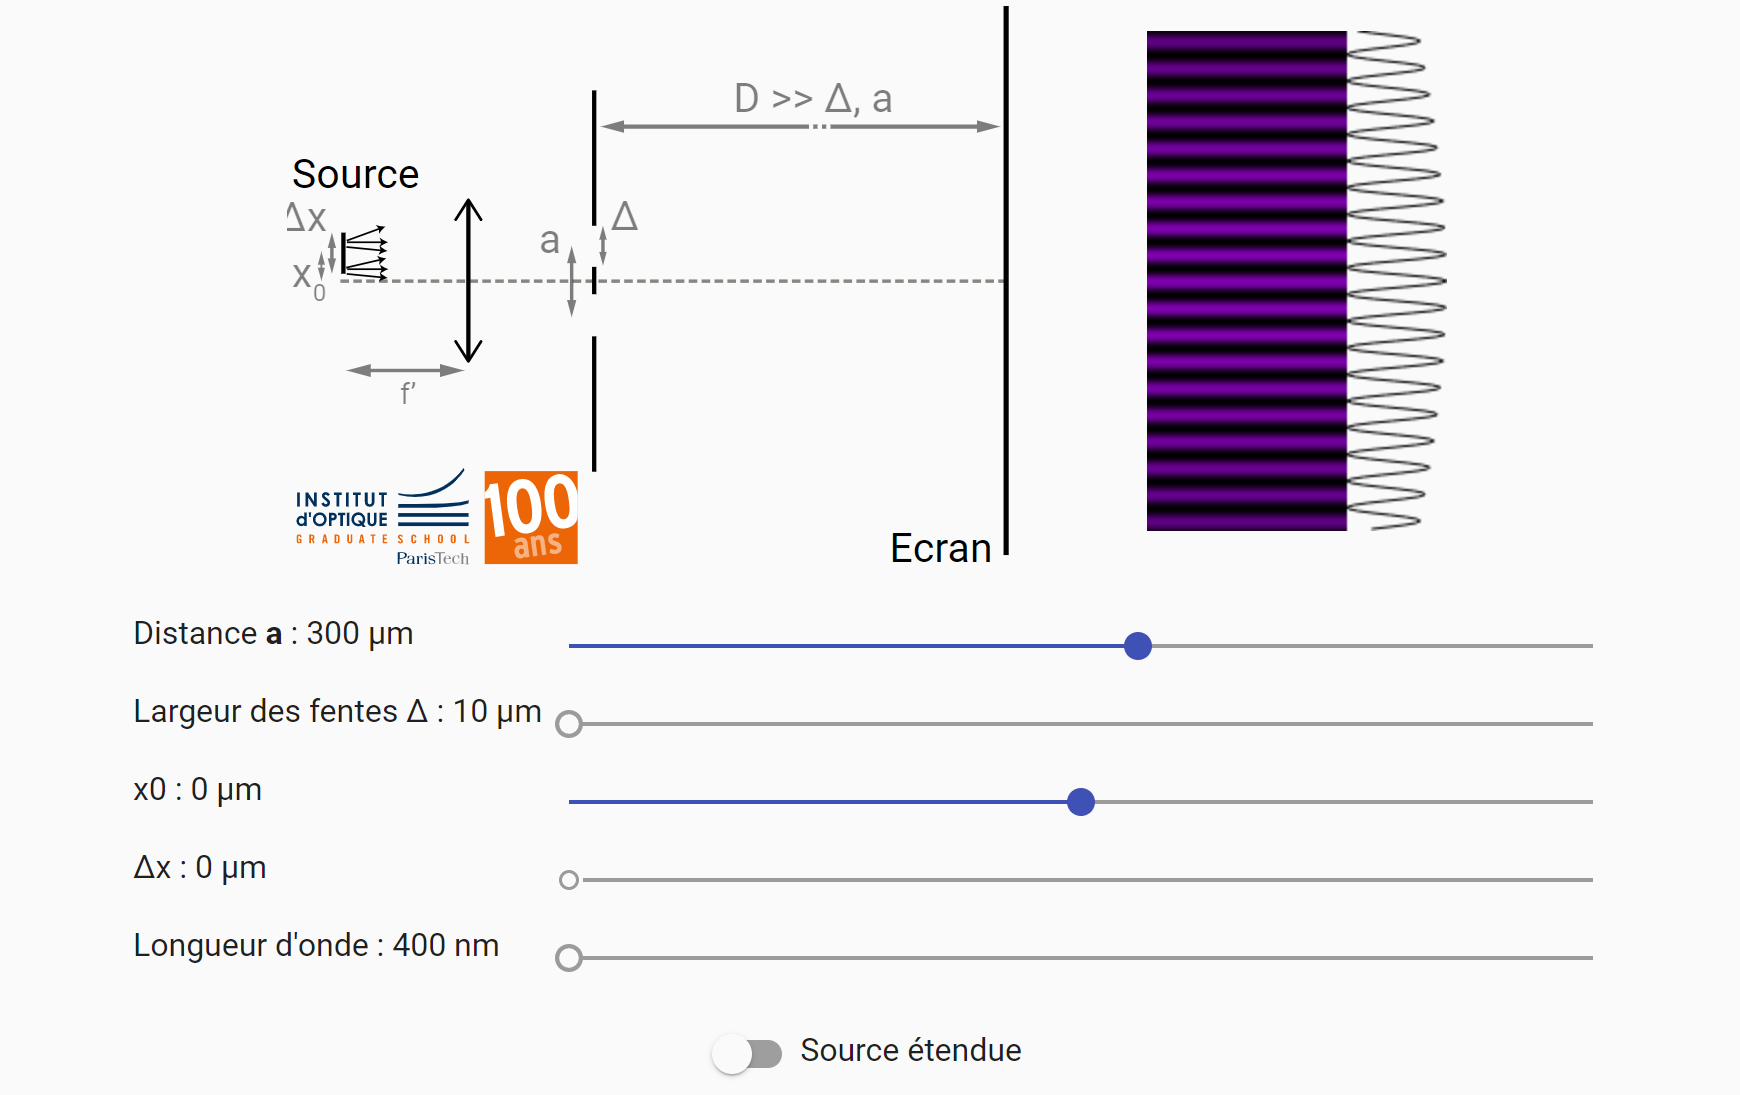
\includegraphics[scale=0.35]{tr6_1.png}
    %\caption{fig1}
    \end{minipage}%
    }%
    \subfigure[$a_2$=150 $\mu m$]{
    \begin{minipage}[t]{0.5\linewidth}
    \centering
    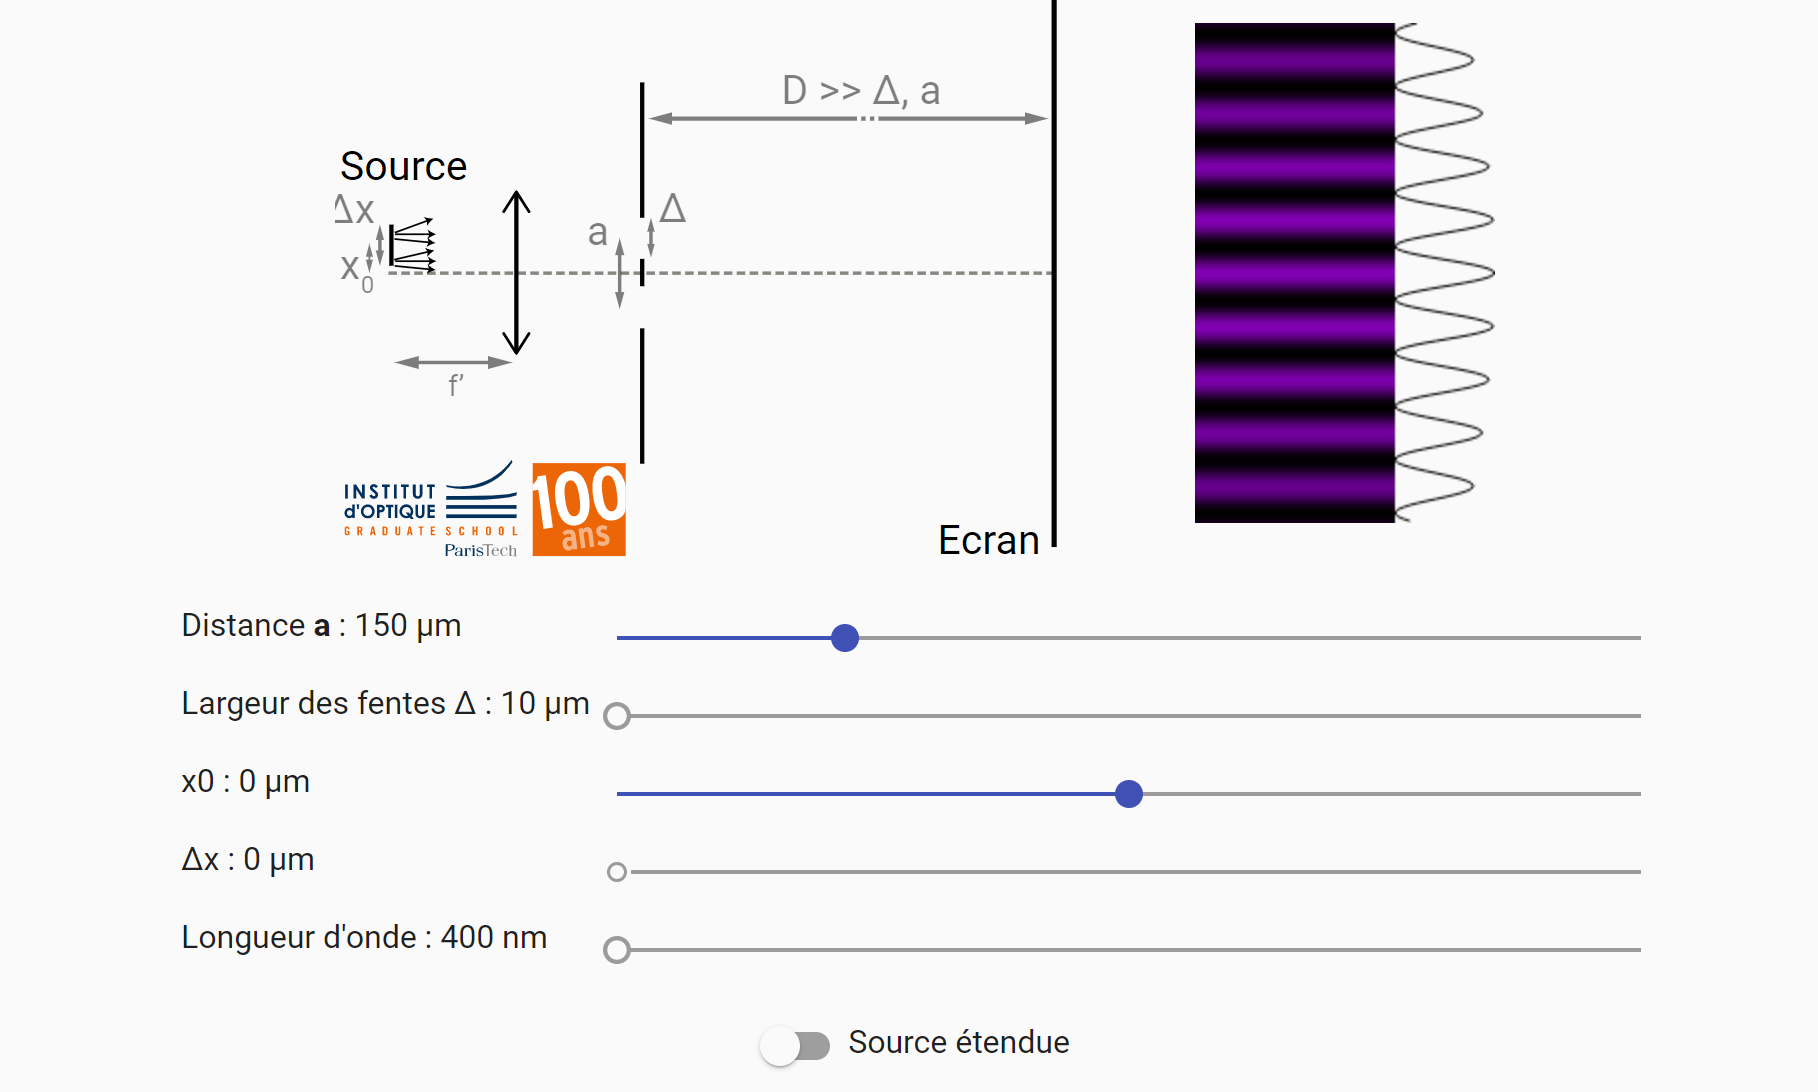
\includegraphics[scale=0.35]{tr6_2.png}
    %\caption{fig2}
    \end{minipage}%
    }%
    \centering
    %\caption{ pics}
    \caption{Changement de distance entre les deux trous}
    \end{figure}

Lorsque on varie le distance $a$ entre les deux trous $S_1, S_2$, avec les autres 
paramètres invariant, on voit que les spectraux deviennent plus gros. 
C'est parce que l'interfrange $i$ entre spectraux brillantes ($resp.$ sombres) adjacents 
est $i=\frac{\lambda_0D}{a}$ par notre approximation dans le cas expérimental.

On a donc $i_1=\frac{\lambda_0D}{a_1}$ et $i_2=\frac{\lambda_0D}{a_2}$, donc 
$\frac{i_1}{i_2}=\frac{a_2}{a_1}=\frac{1}{2}$. Les spectraux pour la figure(b) sont deux fois 
plus gros que ceux pour la figure(a). En fait, il y a $38$ spectraux dans la figure(a), et $19$ 
spectraux dans le figure(b). 


\end{document}